\chapter{Concetti preliminari e tecnologie utilizzate}

\medskip

Vengono di seguito chiariti nel dettaglio i concetti fondamentali necessari a comprendere appieno il progetto presentato in sede di discussione e le tecnologie utilizzate per svilupparlo.

\section{Solid}

\medskip

{\tt Solid}, (Social linked data) è una specifica che permette di salvare i propri dati in sicurezza in data stores decentralizzati chiamati {\tt Pods}. Qualsiasi tipo di informazione può essere salvato in un {\tt  Pod} e l'utente che ne è proprietario può decidere con chi condividere i propri dati, concedendo permessi ad altre applicazioni o ad altri utenti, avendo comunque la possibilità di revocarli in un secondo momento. Ogni {\tt Pod} è interamente controllabile dal proprio proprietario, che può quindi decidere autonomamente come gestirlo. 

\medskip

{\tt Solid} è stato creato da Sir Tim Berners-Lee, fondatore del {\tt World Wide Web}, in collaborazione con il MIT, con il fine di decentralizzare nuovamente il web; quest'ultimo era stato originariamente pensato come un luogo in cui tutti gli utenti avrebbero potuto collaborare per poter creare dati, permettendo loro quindi non solo di leggere i contenuti già esistenti, ma anche di cooperare per crearne dei nuovi. Oggi i dati relativi agli utenti vengono salvati dalle applicazioni, come i social network, in database locali; questo porta ad una serie di svantaggi per l'utente, al quale non è permesso di accedere direttamente ai propri dati.

\bigskip

Quando i dati vengono salvati lontano dagli utenti:

\begin{itemize}
	\item Non si ha quasi nessuna visibilità su ciò che viene conservato.
	\item Si ha scarso controllo su come i dati vengano utlizzati, e su chi vi possa accedere.
	\item Non si può scegliere quali applicazioni usare per poter accedere a tali informazioni.
	\item Non si possono utilizzare i dati come unità coesiva, essendo questi sparsi per il web, sotto il controllo di proprietari differenti e salvati con diversi formati.
\end{itemize}

\medskip

{\tt Solid} mira a risolvere questo problema dividendo il piano dei dati da quello delle applicazioni; in questo modo l'utente è portato a scegliere quale applicazione usare soltanto in base alla qualità dei servizi offerti dall'applicazione stessa e non per il monopolio sul possesso dei dati dell'utente. {\tt Solid} permette quindi ai singoli utenti di tornare ad essere i padroni del web, decentralizzandolo nuovamente, esattamente come era stato pensato in origine da Berners-Lee. Attualmente la tecnologia è ancora in via di sviluppo e i server {\tt Solid} utilizzati, \href{https://inrupt.net/}{https://inrupt.net/} e \href{https://solidcommunity.net/}{https://solidcommunity.net/} non offrono garanzie riguardanti la stabilità e la sicurezza dei dati salvati.

\section{Terminologia Solid}

\medskip

Per poter comprendere appieno la tecnologia {\tt Solid}, è necessario spiegare il significato di alcuni termini connessi con essa.

\medskip
\begin{itemize}
	\item {\tt Pod}: luogo in cui l'utente può scrivere i propri dati personali. Un utente può scegliere di utilizzare uno oppure più {\tt Pod} per memorizzare le proprie informazioni. Le applicazioni possono eseguire diversi tipi di operazioni sui dati dell'utente in relazione ai tipi di permesso che sono stati loro concessi.
	\item {\tt WebId}: un {\tt Internationalised Resource Identifier (IRI)} necessario per identificare univocamente un utente.\\É qui di seguito mostrato un esempio di {\tt webId}:\\
	\href{https://carlotosoni99.inrupt.net/profile/card#me}
	{$https://carlotosoni99.inrupt.net/profile/card\#me$}.
	\item {\tt Pod Provider}: compagnia o organizzazione che permette di ospitare i {\tt Pod} degli utenti.
	\item {\tt Identity Provider}: compagnia o organizzazione che mette a disposizione il servizio di autenticazione con il server {\tt Solid}.
	\item {\tt Solid Identity Provider}: compagnia o organizzazione che è contemporaneamente un {\tt Pod Provider} e un {\tt Identity Provider}.
\end{itemize}

\medskip

Infine vengono dette applicazioni {\tt Solid}, quelle applicazioni che accedono ai dati degli utenti, memorizzati all'interno dei rispettivi {\tt Pod}, utilizzando il {\tt Solid Protocol}
\cite{solidprotocol}, ovvero il protocollo utilizzato da {\tt Solid} per permettere lo scambio di dati, il quale stabilisce che lo scambio di informazione, tra {\tt Solid} app e {\tt Pod}, debba avvenire tramite il protocollo {\tt HTTP}.

\bigskip

\section{Linked Data}

\medskip

Secondo la tecnologia {\tt Solid}, qualisiasi applicazione, se autorizzata dall'utente, deve poter eseguire operazioni sui dati contenuti all'interno del {\tt Pod}. Per questo motivo è necessario che i dati vengano rappresentati tramite un'unica modalità.

\medskip

A tal proposito in {\tt Solid} viene utilizzato il linguaggio {\tt RDF} (Resource Description Framework) per rappresentare i dati contenuti all'interno del {\tt Pod}. Qualsiasi dato in {\tt RDF} viene detto {\tt risorsa}; ogni {\tt risorsa} è rappresentata tramite un {\tt IRI} e pertanto è reperibile direttamente dal web. Oltre alle {\tt risorse}, il modello di dati {\tt RDF} è formato anche da {\tt proprietà} e {\tt valori}: le prime sono relazioni che permettono di collegare {\tt risorse} e {\tt valori}; un {\tt valore} invece è la valenza della {\tt risorsa} per tale {\tt proprietà}; eventualmente un {\tt valore} può essere un dato primitivo, come, ad esempio, una stringa. Le {\tt risorse} vengono infine descritte in {\tt vocabolari}, i quali a loro volta sono rappresentati tramite {\tt IRI}. All'interno di un {\tt vocabolario} vengono definite {\tt classi} e {\tt proprietà}, le {\tt classi} sono utilizzate per indicare il tipo di dato che si vuole rappresentare, le {\tt proprietà} sono semplicemente attributi relativi a istanze di una classe; visitando l'{\tt IRI} relativo ad un {\tt vocabolario}, si può trovare la documentazione necessaria per rappresentare un qualche tipo di informazione tramite le {\tt proprietà} e le {\tt classi} definite in tale vocabolario.

\medskip

Spesso per la rappresentazione di dati si utilizzano dei vocabolari noti che ricorrono frequentemente in {\tt Solid}, come ad esempio:

\begin{itemize}
	\item {\tt RDF}: {\tt vocabolario} fondamentale per {\tt RDF}, definisce un modello per rappresentare dati in {\tt RDF}:
	per esempio {\tt rdfs:Class} è la {\tt classe} di {\tt risorse} per rappresentare classi {\tt RDF}, mentre {\tt rdf:Property} è la {\tt classe} delle proprietà {\tt RDF}.
	\item {\tt FOAF} (Friend of a Friend): usato per rappresentare persone e organizzazioni, definisce i termini per rappresentare il profilo di un utente e le interazioni tra gli utenti.
	\item {\tt ACL} (Access Control List): {\tt vocabolario} essenziale per {\tt Solid}, definisce i livelli di accesso di un agente, stabilendo se esso è autorizzato a compiere una determinata operazione.
	\item {\tt Schema}: vocabolario che definisce varie strutture di dati da poter utilizzare nel web.
\end{itemize}

In generale, se per rappresentare un qualche tipo di dato non dovesse esistere un adeguato {\tt vocabolario}, è possibile crearne uno e pubblicarlo nel proprio {\tt Pod}, cosicché anche altri utenti possano utilizzarlo. Per ulteriori informazioni relative ai {\tt vocabolari} è possibile consultare il sito web di {\tt Solid} dove è presente un tutorial per imparare a comprenderne il significato.

\smallskip

\href{https://solidproject.org/developers/vocabularies}{https://solidproject.org/developers/vocabularies}

\medskip

In {\tt RDF} qualsiasi informazione deve essere rappresentata tramite uno {\tt statement}, il quale è definito come una tripla composta da {\tt soggetto}, {\tt predicato} e {\tt oggetto}. Gli {\tt statement} permettono di rappresentare in maniera semplice qualsiasi tipo di informazione. Qui seguito è riportato un esempio di {\tt statement}.

\medskip
\begin{lstlisting}

<https://carlotosoni99.inrupt.net/profile/card#me> (soggetto)
<http://xmlns.com/foaf/0.1/name> (predicato)
"Carlo" (oggetto)


\end{lstlisting}

\medskip

Questa tripla sta a indicare che l'oggetto\\$https://carlotosoni99.inrupt.net/profile/card\#me$, che rappresenta il profilo di un utente in {\tt Solid}, ha una proprietà descritta nel {\tt vocabolario} {\tt FOAF} per rappresentare il nome di una generica persona o organizzazione, e che tale nome è pari a $"Carlo"$, il quale è semplicemente una stringa.

\begin{figure}[ht]
	\centering
	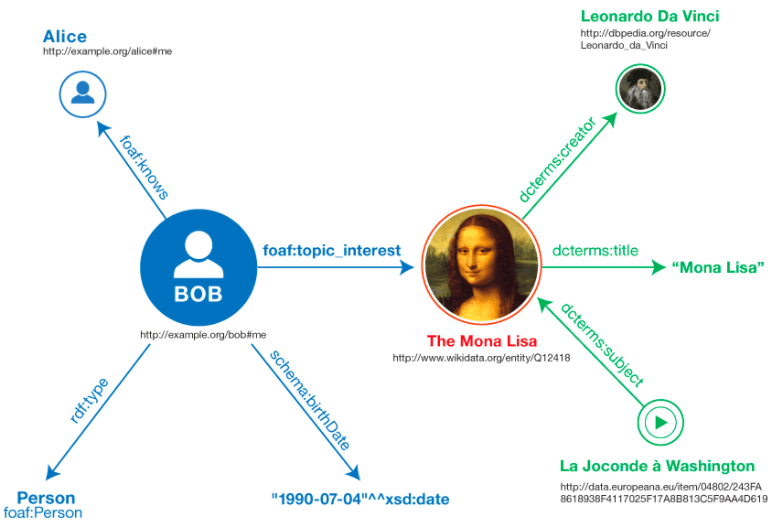
\includegraphics[width=0.87
	\textwidth,  keepaspectratio]{fig/linkedData}
	\caption{Esempio di dati rappresentati in {\tt RDF}}
	\label{fig:linkedData}
\end{figure}

\medskip

Questa modalità di rappresentare i dati viene chiamata anche {\tt Linked Data}, poiché {\tt oggetti} o {\tt classi} appartenti a {\tt vocabolari} differenti, possono essere facilmente connessi tra loro con il fine di rappresentare strutture di dati più complesse.

\medskip

I dati in {\tt RDF} possono essere espressi tramite diverse sintassi; quella mostrata in questa tesi e utilizzata da {\tt Solid}, prende il nome di {\tt Turtle} ("Terse RDF Triple Language"); i file {\tt Turtle} utilizzano il formato {\tt .ttl}. Alcuni dei possibili tipi di dati salvabili in un {\tt Pod} tramite {\tt Turtle} sono: {\tt Url, Boolean, Date, Decimal, Integer, String} e altri.

\bigskip

\section{Struttura di un Pod}

\medskip 

Per poter comprendere appieno il funzionamento dell'applicazione creata come progetto di tesi, è necessario conoscere come è strutturato un {\tt Pod}. Innanzitutto un {\tt Pod} è formato da {\tt containers} e da {\tt risorse}: i {\tt containers} sono degli oggetti simili a delle cartelle che contengono le {\tt risorse};
il {\tt Pod} di un utente è infatti gestito in maniera simile ad un file system di un calcolatore. Le {\tt risorse} invece vanno intese come l'insieme di oggetti e delle loro proprietà, espresse in linguaggio {\tt RDF}, che servono a descrivere la informazioni contenute nel {\tt Pod}.

\medskip

Per esempio all'interno di ciascun {\tt Pod} è presente il {\tt container} {\tt profile}, il quale contiene le informazioni relative al profilo dell'utente possessore del {\tt Pod}.

\medskip

\href{https://carlotosoni99.inrupt.net/profile/}{$https://carlotosoni99.inrupt.net/profile/$}

\medskip

Visitando questo link è possibile vedere che all'interno di questo {\tt container} si trova una risorsa chiamata {\tt card}, nella quale sono presenti tutte le informazioni di interesse dell'utente. In particolare in questo {\tt dataset} è collocato un oggetto avente {\tt IRI} pari a:

\medskip

\href{https://carlotosoni99.inrupt.net/profile/card\#me}{$https://carlotosoni99.inrupt.net/profile/card\#me$}

\medskip

Questo oggetto serve a rappresentare tutte le informazioni più rilevanti riguardanti il {\tt Pod} e il suo utente; da notare che l'{\tt URL} di questo oggetto corrisponde con la {\tt webId} dell'utente stesso. Ogni utente può liberamente leggere il {\tt SolidDataset} {\tt card} anche senza essersi autenticato con il {\tt Solid Identity Provider}.

\medskip

All'interno di un {\tt Pod} esistono altri {\tt containers} e altre {\tt risorse}, oltre a quelli già elencati, che servono a memorizzare differenti tipi di informazioni. In generale, comunque, ogni utente avente diritto di scrittura è libero di aggiungere {\tt containers} e {\tt risorse} all'interno di un {\tt Pod}, per poterlo gestire in base alle proprie necessità.

\medskip

L'applicazione \href{https://podbrowser.inrupt.com/}{$https://podbrowser.inrupt.com/$} sviluppata da {\tt Inrupt}, società fondata da Berners-Lee, permette di vedere il contenuto del proprio {\tt Pod} in maniera user friendly, potendo visualizzare la struttura di {\tt containers} e le rispettive {\tt risorse} al loro interno.

\bigskip

\section{Tipologie di permesso in Solid}

\medskip

In {\tt Solid} non tutti gli utenti sono autorizzati a modificare le risorse contenute all'interno di un {\tt Pod}; il {\tt vocabolario} {\tt ACL} (access control list), già enunciato, viene utilizzato per determinare se un utente è autorizzato o meno a compiere una determinata operazione. Il vocabolario {\tt ACL} descrive quattro diversi tipologie di permessi:

\medskip

\begin{itemize}
	\item {\tt Read}: permesso in lettura su una {\tt risorsa}.
	\item {\tt Append}: permesso di aggiungere ulteriori informazioni ad una {\tt risorsa} già\\ esistente, senza poterla eliminare.
	\item {\tt Write}: permesso di eseguire operazioni in scrittura su una {\tt risorsa}, potendo creare, modificare o eliminare una determinata {\tt risorsa} nel {\tt Pod}.
	\item {\tt Control}: permesso di eseguire operazioni in lettura e scrittura su un file {\tt ACL} correlato con una {\tt risorsa}.
\end{itemize}

\medskip

Nel momento in cui ci si autentica nel proprio {\tt Pod} tramite un'applicazione {\tt Solid} per la prima volta, viene data all'utente la possibilità di scegliere quali debbano essere i permessi di tale applicazione sulle {\tt risorse} presenti all'interno del proprio {\tt Pod}. Tali permessi possono essere eventualmente revocati in un secondo momento.

\medskip

Inoltre modificando le {\tt risorse ACL} presenti all'interno del proprio {\tt Pod}, è possibile andare a personalizzare le tipologie di permesso dell'applicazione sulle singole {\tt risorse} presenti.
\medskip

Per ulteriori chiarimenti riguardanti il sistema di autorizzazione usato da {\tt Solid} è possibile leggere il documento {\tt Web Access Control} \cite{wac}.

\bigskip

\section{Autenticazione in Solid}

\medskip

Spesso le applicazioni {\tt Solid} necessitano di autenticarsi con il/i {\tt Solid Identity Provider} appartente/i all'/agli utente/i in questione; tale operazione è spesso necessaria per poter ottenere i permessi necessari all'applicazione per poter interagire con le {\tt risorse} contenute all'interno dei {\tt Pod}. A seguito dell'operazione di autenticazione, le applicazioni {\tt Solid} vengono quindi autorizzate dal {\tt Solid Identity Provider} ad eseguire alcune operazioni sui dati dell'utente in base alle tipologie di permesso concesse.

\medskip

{\tt Inrupt} mette a disposizione una serie di librerie che permettono di autenticarsi con il proprio {\tt Solid Identity Provider} da Browser oppure tramite {\tt Node.js}.

\medskip

Utilizzando le librerie {\tt Inrupt} la procedura di autenticazione è relativamente semplice da eseguire: è necessario innanzitutto indicare il proprio {\tt Solid Identity Provider}, dopodiché l'utente viene indirizzato presso di questo per completare l'operazione di autenticazione con i propri dati (username e password); una volta terminata questa operazione l'utente è reindirizzato all'applicazione che stava utilizzando.

\medskip

Per ulteriori informazioni riguardanti il processo di autenticazione in {\tt Solid}, è possibile visitare la seguente pagina:\\
\href{https://solid.github.io/authentication-panel/solid-oidc/}{https://solid.github.io/authentication-panel/solid-oidc/}.

\bigskip

\section{Ulteriori chiarimenti riguardo la tecnologia Solid}

\bigskip

Qui di seguito vengono ora espressi nel dettaglio ulteriori concetti relativi alla tecnologia {\tt Solid}, i quali sono utili per comprendere in maniera più approfondita il progetto.

\bigskip

{\tt Solid} è una tecnologia che non si pone l'obiettivo di reinventare il web, ma che mira ad aggiungere a questo alcune caratteristiche, come la presenza di un sistema di identificazione per evitare di dover creare un account su ogni piattaforma presente all'interno della rete, come Facebook, Twitter, Google e molte altre. Obiettivo di {\tt Solid} è inoltre la possibilità di permettere ai vari social media, di condividere i dati relativi ai singoli utenti, indipendente dal tipo di social media utilizzato. Le applicazioni {\tt Solid} possono funzionare correttamente anche senza salvare in database locali alcun dato relativo ai singoli utenti; infatti come già detto, tutti i dati vengono salvati all'interno dei {\tt Pod} degli utenti. {\tt Solid} inoltre mette a disposizione dell'utente la possibilità di ospitare il proprio {\tt Pod} all'interno del suo hard disk o server, senza doversi affidare ad un {\tt Solid Identity Provider}. É anche possibile, quindi, divenire un piccolo {\tt Pod Provider} o {\tt Identity Provider}, con il fine di ospitare i {\tt Pod} appartenti, per esempio, alla propria famiglia, o ai membri dell'organizzazione di cui si fa parte. Un utente può inoltre possedere più di un {\tt Pod} contemporaneamente e salvare su ognuno di essi differenti tipologie di dati in relazione alle proprie necessità; inoltre sussiste la possibilità di cambiare {\tt Pod Provider} in un secondo momento, recuperando i dati presenti all'interno del {\tt Pod}.

\bigskip
\medskip

Riguardo al sistema di identificazione presente in {\tt Solid}, una {\tt webId} non deve\\ necessariamente essere usata per identificare una persona fisica, bensì può riferirsi anche a organizzazioni, compagnie, famiglie, team o, più generalmente, a qualsiasi gruppo di persone.

\bigskip
\medskip

Per quanto concerne la sicurezza dei dati salvati all'interno del proprio {\tt Pod} è bene fare alcune precisazioni. Innanzitutto il livello di sicurezza dei propri dati dipende dal {\tt Pod Provider} utilizzato; i {\tt Pod Provider}, in generale, non hanno vincoli riguardanti la crittografia utilizzata per criptare i dati contenuti all'interno del {\tt Pod}. L'utente ha il compito di scegliere un {\tt Pod Provider} che cripti i propri dati adeguatamente se la sicurezza di questi è importante per lui. Infine, poiché {\tt Solid} non prevede che i dati relativi ad un utente debbano essere necessariamente salvati all'interno di un singolo luogo, essendo possibile utilizzare più di un {\tt Pod} per la memorizzazione delle proprie informazioni, {\tt Solid} non rende gli utenti maggiormente vulnerabili da parte di attacchi informatici. A tal proposito è necessario considerare anche che attacchi informatici da parte di hackers sono maggiormente probabili se riferiti a una singola fonte di dati di molte persone, piuttosto che a livello individuale.



\bigskip
\bigskip
\bigskip
\bigskip

All'interno del sito web \href{https://solidproject.org/}{https://solidproject.org/} sono presenti ulteriori informazioni, per sviluppatori e non, riguardanti il progetto {\tt Solid}.

\bigskip

\section{Inrupt}

\medskip

{\tt Inrupt} è una società fondata da Sir Tim Berners-Lee nel 2018 per fornire strumenti atti a favorire lo sviluppo di {\tt Solid}. Secondo Berners-Lee, {\tt Inrupt} mira a "fornire energia commerciale e un ecosistema per aiutare a proteggere l'integrità e la qualità del nuovo web costruito su Solid" \cite{inrupt}.

\medskip

In particolare {\tt Inrupt} fornisce una serie di strumenti per potersi autenticare con il proprio {\tt Solid Identity Provider} e per poter aggiungere, creare, modificare e cancellare le informazioni all'interno del proprio {\tt Pod}.

\medskip

Le librerie create da {\tt Inrupt}, e usate anche nel progetto oggetto della tesi, sono:

\begin{itemize}
	\item {\tt solid-client-authn-browser}: tale libreria permette di autenticarsi con il proprio {\tt Solid Identity Provider} tramite browser.
	\item {\tt solid-client-authn-node}: questa libreria permette di autenticarsi con il proprio {\tt Solid Identity Provider} tramite Node.js.
	\item {\tt solid-ui-react}: mette a disposizione componenti per applicazioni in React per potersi autenticare con il proprio {\tt Solid Identity Provider} e per poter leggere e scrivere le informazioni contenute all'interno del {\tt Pod}.
	\item {\tt solid-client}: fornisce funzioni atte a eseguire ogni possibile azione all'interno del proprio {\tt Pod}, tra le quali: scaricare {\tt SolidDataset} presenti all'interno del proprio {\tt Pod}, modificare un {\tt SolidDataset} già esistente o crearne uno all'interno del proprio {\tt Pod}, caricare, modificare un {\tt oggetto} appartenente ad un determinato {\tt SolidDataset}, oppure crearne uno nuovo, leggere gli {\tt statement} di un {\tt oggetto} per poter ricavare informazioni presenti nel proprio {\tt Pod}, oppure modificare {\tt statement} già esistenti o crearne dei nuovi, leggere e scrivere {\tt risorse ACL} e utilizzare altre funzionalità.
\end{itemize}

\medskip

Le librerie messe a disposizioni da {\tt Inrupt} sono attualmente le più utilizzate per programmare applicazioni in {\tt Solid}. Oltre a questo, {\tt Inrupt} gestisce uno dei due {\tt Solid Identity Provider} più utilizzati al momento;\\
visitando il seguente URL si può accedere al sito \href{https://inrupt.net/}{https://inrupt.net/} per potersi\\registrare con il {\tt Solid Identity Provider} e creare un proprio {\tt Pod}.

\medskip

Per leggere la documentazione relativa alle librerie sopra enunciate è possibile\\visitare i seguenti URL:

{\tt solid-client-authn-browser} e {\tt solid-client-authn-node}:\\ \href{https://docs.inrupt.com/developer-tools/javascript/client-libraries/authentication/}{https://docs.inrupt.com/developer-tools/javascript/client-libraries/authentication/}\\
{\tt solid-ui-react}:\\ \href{https://solid-ui-react.docs.inrupt.com/?path=/story/intro--page}{https://solid-ui-react.docs.inrupt.com/?path=/story/intro--page} \\
{\tt solid-client}:\\
\href{https://docs.inrupt.com/developer-tools/javascript/client-libraries/tutorial/read-write-data/}{https://docs.inrupt.com/developer-tools/javascript/client-libraries/tutorial/read-write-data/} e\\
\href{https://docs.inrupt.com/developer-tools/api/javascript/solid-client/}{https://docs.inrupt.com/developer-tools/api/javascript/solid-client/}

\medskip

\section{React}

\medskip

{\tt React} è una libreria {\tt open-source}, {\tt front-end}, {\tt JavaScript}, finalizzata alla creazione di interfacce utente ed attualmente molto conosciuta e usata. Vengono qui elencate le caratteristiche principali di {\tt React}:

\medskip 

\begin{itemize}
	\item Permette di creare interfacce grafiche in maniera semplificata. Le interfacce sono progettate per ogni stato dell'applicazione; ad ogni cambio di stato {\tt React} aggiorna solo le parti delle UI che dipendono da tali dati.
	\item Agevola la creazione di interfacce grafiche complesse, permettendo di creare componenti in isolamento e ricomponibili per formare UI complesse.
	\item {\tt React} non è dipendente da altre tecnologie: in questo modo si possono sviluppare nuove funzionalità in {\tt React} senza dover riscrivere qualsiasi codice già esistente.
\end{itemize}

\medskip

{\tt JSX} è la sintassi che {\tt React} utilizza per descrivere l'aspetto delle interfacce grafiche. Comunque l'utilizzo di {\tt JSX}, pur essendo raccomandato, risulta opzionale e non richiesto per programmare in {\tt React}. {\tt JSX} va inteso come un'estensione della sintassi di {\tt Javascript}, riprendendo le proprie caratteristiche sia da {\tt Javascript} stesso che da {\tt HTML}.

\bigskip

L'applicazione {\tt my-solid-blog} è stata sviluppata utilizzando {\tt React} e, in particolare, il comando {\tt create-react-app} di {\tt npx}, il quale permette di creare applicazioni in {\tt React} single-page. {\tt create-react-app} crea autonomamente un ambiente di sviluppo che consente di utilizzare le caratteristiche più recenti di {\tt JavaScript}, utilizzando, per esempio, {\tt Babel} e {\tt webpack}.

\bigskip

Le motivazioni che hanno portato a sviluppare {\tt my-solid-blog} in {\tt React} sono principalmente due: la prima è che la libreria {\tt solid-ui-react} di {\tt Inrupt} permette ad applicazioni in {\tt React} di gestire alcune operazioni in {\tt Solid}, come l'autenticazione con {\tt Solid Identity Provider}, in maniera semplice e intuitiva; il secondo motivo riguarda la semplicità con cui {\tt React} permette agli sviluppatori di creare e gestire interfacce grafiche. Per renderizzare le proprie interfacce grafiche, l'applicazione {\tt my-solid-blog} utilizza la sintassi {\tt JSX}. Le applicazioni {\tt React} create tramite comando {\tt create-react-app} possono essere avviate in {\tt development mode} utilizzando il comando {\tt npm start}.

\bigskip

Per ulteriori informazioni relative alla libreria {\tt React} è possibile visitare il sito web:

\smallskip

\href{https://it.reactjs.org/}{https://it.reactjs.org/}.

\bigskip

\section{Bulma}

\medskip

{\tt Bulma} è un framework {\tt CSS} {\tt open source} che si è particolarmente diffuso negli ultimi anni, raggiungendo 40.000 stelle su {\tt GitHub}. È caratterizzato da una sintassi semplice che permette di importare nei propri progetti vari componenti predefiniti; {\tt Bulma} presenta un design minimalista e unico nel suo genere, capace di rendere maggiormente accattivamente una pagina web.

\bigskip

Il framework {\tt Bulma} è stato scelto per gestire il layout dell'applicazione\\{\tt my-solid-blog} per la sua semplicità, per il suo design e per la compatibilità con la libreria {\tt React}.

\medskip

Visitando il seguente URL è possibile leggere la documentazione relativa a {\tt Bulma}:

\smallskip

\href{https://bulma.io/}{https://bulma.io/}

\bigskip

\section{Node.js}

\medskip

{\tt Node.js} è un {\tt runtime system} {\tt open source} multipiattaforma {\tt orientato agli eventi}. Quando è stato introdotto, {\tt Node.js} ha consentito l'esecuzione di codice {\tt JavaScript} da {\tt lato server}; precedentemente {\tt JavaScript} era stato utilizzato principalmente da {\tt lato Client}. Data la sua enorme potenzialità, {\tt Node.js} è attualmente una delle tecnologie più richieste sul mercato del lavoro.

\bigskip

All'interno di questo progetto {\tt Node.js} è stato utlizzato per sviluppare l'applicazione {\tt blog-validator}, con lo scopo di effettuare alcuni controlli sui dati presenti nel {\tt Pod}. Tale server si occupa infatti di verificare l'autenticità dei dati mostrati dall'applicazione {\tt my-solid-blog} su richiesta dell'utente.

\clearpage

\section{Altri strumenti utilizzati}

\bigskip

\textbf{Axios}

\bigskip

{\tt Axios} è una libreria che permette di inviare richieste {\tt HTTP} da browser o da {\tt Node.js}. Tale libreria è stata utilizzata per permettere la trasmissione di informazioni tra l'applicazione {\tt my-solid-blog} e il server {\tt Node.js}, con il fine di comunicare al server alcune informazioni relative ai contenuti mostrati all'interno dell'applicazione stessa.

\smallskip

\href{https://github.com/axios/axios}{https://github.com/axios/axios}

\bigskip

\textbf{vocab-common-rdf e rdf-namespaces}

\bigskip

Queste due librerie di {\tt JavaScript} contengono degli pseudonimi per i vocabolari {\tt RDF} più utilizzati, permettendo di utilizzare {\tt proprietà} e {\tt classi} di alcuni vocabolari {\tt RDF} in maniera semplificata e snellendo il codice dell'applicazione.

\medskip

Ad esempio la libreria {\tt rdf-namespaces} permette di utilizzare la proprietà {\tt type} del vocabolario {\tt http://www.w3.org/1999/02/22-rdf-syntax-ns} semplicemente scrivendo {\tt rdf.type}, anziché\\{\tt http://www.w3.org/1999/02/22-rdf-syntax-ns\#type}.

\medskip

Tale proprietà, fondamentale nel linguaggio {\tt RDF}, è utilizzata per indicare che una {\tt risorsa} è un'instanza di una {\tt classe}.

\clearpage